\hypertarget{stm32f4xx__hal__gpio_8c}{}\section{Dokumentacja pliku S\+T\+M/\+W\+D\+S\+\_\+\+Kosc\+\_\+\+Linux/\+Drivers/\+S\+T\+M32\+F4xx\+\_\+\+H\+A\+L\+\_\+\+Driver/\+Src/stm32f4xx\+\_\+hal\+\_\+gpio.c}
\label{stm32f4xx__hal__gpio_8c}\index{S\+T\+M/\+W\+D\+S\+\_\+\+Kosc\+\_\+\+Linux/\+Drivers/\+S\+T\+M32\+F4xx\+\_\+\+H\+A\+L\+\_\+\+Driver/\+Src/stm32f4xx\+\_\+hal\+\_\+gpio.\+c@{S\+T\+M/\+W\+D\+S\+\_\+\+Kosc\+\_\+\+Linux/\+Drivers/\+S\+T\+M32\+F4xx\+\_\+\+H\+A\+L\+\_\+\+Driver/\+Src/stm32f4xx\+\_\+hal\+\_\+gpio.\+c}}


G\+P\+IO H\+AL module driver. This file provides firmware functions to manage the following functionalities of the General Purpose Input/\+Output (G\+P\+IO) peripheral\+:  


{\ttfamily \#include \char`\"{}stm32f4xx\+\_\+hal.\+h\char`\"{}}\newline
Wykres zależności załączania dla stm32f4xx\+\_\+hal\+\_\+gpio.\+c\+:\nopagebreak
\begin{figure}[H]
\begin{center}
\leavevmode
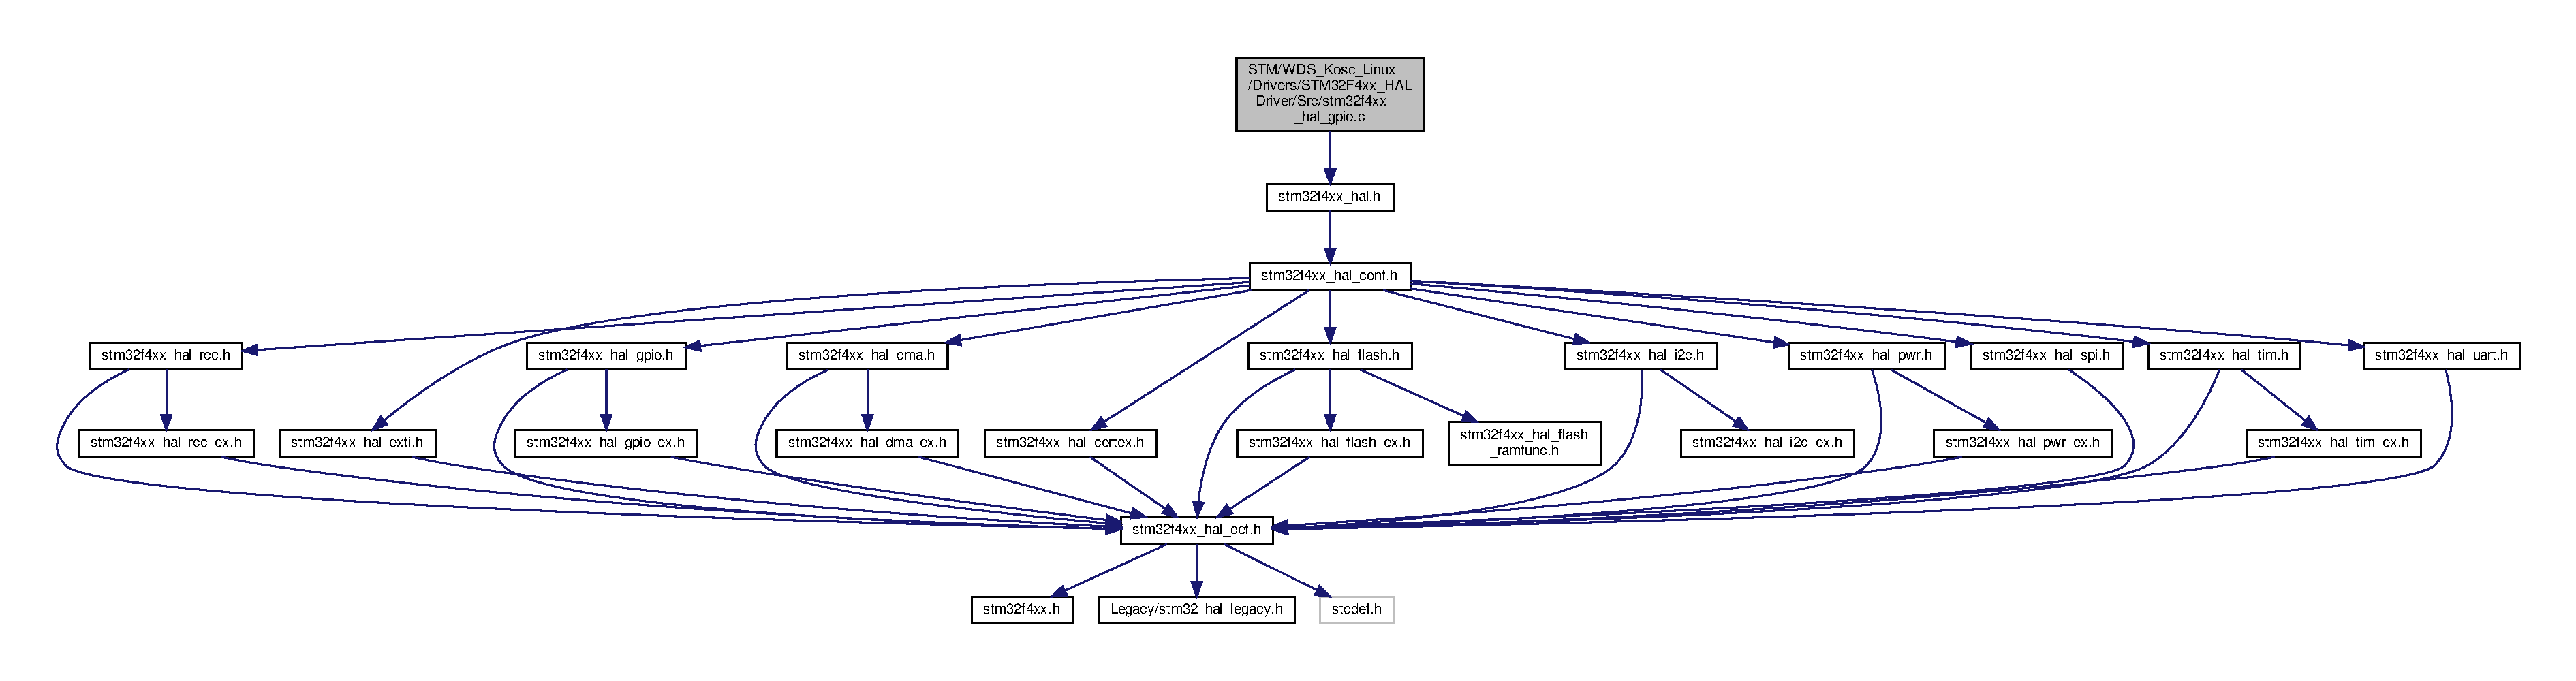
\includegraphics[width=350pt]{stm32f4xx__hal__gpio_8c__incl}
\end{center}
\end{figure}


\subsection{Opis szczegółowy}
G\+P\+IO H\+AL module driver. This file provides firmware functions to manage the following functionalities of the General Purpose Input/\+Output (G\+P\+IO) peripheral\+: 

\begin{DoxyAuthor}{Autor}
M\+CD Application Team
\begin{DoxyItemize}
\item Initialization and de-\/initialization functions
\item IO operation functions
\end{DoxyItemize}
\end{DoxyAuthor}
\begin{DoxyVerb}==============================================================================
                  ##### GPIO Peripheral features #####
==============================================================================
[..] 
Subject to the specific hardware characteristics of each I/O port listed in the datasheet, each
port bit of the General Purpose IO (GPIO) Ports, can be individually configured by software
in several modes:
(+) Input mode 
(+) Analog mode
(+) Output mode
(+) Alternate function mode
(+) External interrupt/event lines

[..]  
During and just after reset, the alternate functions and external interrupt  
lines are not active and the I/O ports are configured in input floating mode.

[..]   
All GPIO pins have weak internal pull-up and pull-down resistors, which can be 
activated or not.

[..]
In Output or Alternate mode, each IO can be configured on open-drain or push-pull
type and the IO speed can be selected depending on the VDD value.

[..]  
All ports have external interrupt/event capability. To use external interrupt 
lines, the port must be configured in input mode. All available GPIO pins are 
connected to the 16 external interrupt/event lines from EXTI0 to EXTI15.

[..]
The external interrupt/event controller consists of up to 23 edge detectors 
(16 lines are connected to GPIO) for generating event/interrupt requests (each 
input line can be independently configured to select the type (interrupt or event) 
and the corresponding trigger event (rising or falling or both). Each line can 
also be masked independently. 

                   ##### How to use this driver #####
==============================================================================  
[..]
  (#) Enable the GPIO AHB clock using the following function: __HAL_RCC_GPIOx_CLK_ENABLE(). 

  (#) Configure the GPIO pin(s) using HAL_GPIO_Init().
      (++) Configure the IO mode using "Mode" member from GPIO_InitTypeDef structure
      (++) Activate Pull-up, Pull-down resistor using "Pull" member from GPIO_InitTypeDef 
           structure.
      (++) In case of Output or alternate function mode selection: the speed is 
           configured through "Speed" member from GPIO_InitTypeDef structure.
      (++) In alternate mode is selection, the alternate function connected to the IO
           is configured through "Alternate" member from GPIO_InitTypeDef structure.
      (++) Analog mode is required when a pin is to be used as ADC channel 
           or DAC output.
      (++) In case of external interrupt/event selection the "Mode" member from 
           GPIO_InitTypeDef structure select the type (interrupt or event) and 
           the corresponding trigger event (rising or falling or both).

  (#) In case of external interrupt/event mode selection, configure NVIC IRQ priority 
      mapped to the EXTI line using HAL_NVIC_SetPriority() and enable it using
      HAL_NVIC_EnableIRQ().
       
  (#) To get the level of a pin configured in input mode use HAL_GPIO_ReadPin().
          
  (#) To set/reset the level of a pin configured in output mode use 
      HAL_GPIO_WritePin()/HAL_GPIO_TogglePin().
  
  (#) To lock pin configuration until next reset use HAL_GPIO_LockPin().

               
  (#) During and just after reset, the alternate functions are not 
      active and the GPIO pins are configured in input floating mode (except JTAG
      pins).

  (#) The LSE oscillator pins OSC32_IN and OSC32_OUT can be used as general purpose 
      (PC14 and PC15, respectively) when the LSE oscillator is off. The LSE has 
      priority over the GPIO function.

  (#) The HSE oscillator pins OSC_IN/OSC_OUT can be used as 
      general purpose PH0 and PH1, respectively, when the HSE oscillator is off. 
      The HSE has priority over the GPIO function.\end{DoxyVerb}


\begin{DoxyAttention}{Uwaga}

\end{DoxyAttention}
\subsubsection*{\begin{center}\copyright{} Copyright (c) 2017 S\+T\+Microelectronics. All rights reserved.\end{center} }

This software component is licensed by ST under B\+SD 3-\/\+Clause license, the \char`\"{}\+License\char`\"{}; You may not use this file except in compliance with the License. You may obtain a copy of the License at\+: opensource.\+org/licenses/\+B\+S\+D-\/3-\/\+Clause 